\chapter{The Gathering}
\label{ch:03}



\begin{center}
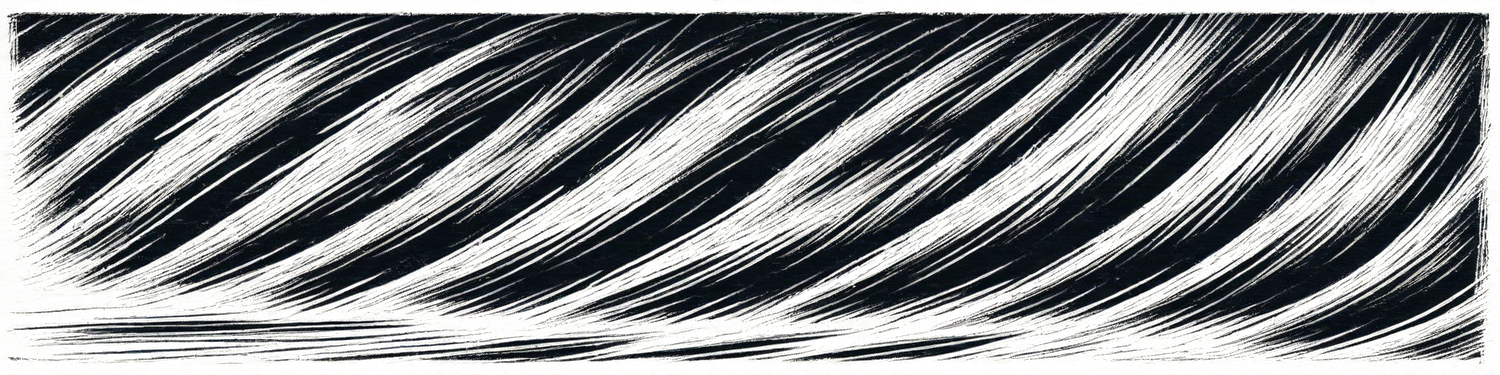
\includegraphics[width=\textwidth]{images/chapterImages/genesis_sketch_00056_.png}
\end{center}

Aurelia's hollow tree stood at the edge of a ravine where water had carved deep channels over millennia. Three young ones slept inside with her, their smaller bodies pressed against her flanks for warmth. They were past the helpless stage but not yet independent, still learning the basic calculus of survival: where to hunt, how to avoid larger predators, which plants indicated good water sources.

She woke before dawn as always, the internal timing precise. The young ones stirred when she moved but didn't wake. She slipped from the hollow carefully, disturbing them as little as possible.

Outside, frost coated the ferns. The temperature had dropped sharply overnight. She paid it no attention beyond the automatic adjustments her body made—feathers fluffing slightly for better insulation, metabolism increasing a fraction.

At the base of the tree, cached in a crevice of roots, was food she hadn't placed there. A small mammal, freshly killed within the last few hours. The killing bite was efficient, precise. She recognized the technique without conscious thought—the same technique she used herself. Someone of her kind had left this.

She ate half of it, methodically, wasting nothing. Cached the rest for the young ones. Then she moved toward her clearing.

The three stones remained exactly as she'd placed them. She stood in their center and looked up at the sky, finding the star point in the pre-dawn darkness. It was brighter. Measurably so. The change was small but definite.

She ran the calculations again, integrating the new data. The trajectory held. The timing compressed slightly—not by much, but enough to register. Enough to require response.

She needed to be elsewhere today.

When she returned to the hollow, the young ones were awake, making small chirping sounds that they would grow out of in another season. They tumbled toward her, hungry, demanding. She led them to the cached food and watched as they tore into it with juvenile inefficiency. They would need to learn better technique. Later. There was always later for teaching the small skills.

Until there wasn't.

At the ravine's edge, another presence. The one who had been leaving food—she recognized him now, though they had never directly interacted. He stood at a respectful distance, not approaching, not threatening. Just present.

She looked at him for several seconds. He didn't move. Didn't display submission or dominance. Just stood.

The young ones noticed him and tensed, their limited instincts uncertain whether this represented danger. She made a small sound—not quite vocalization, more of an exhaled click—and they relaxed slightly.

The other one lowered his head in what might have been a nod or might have been simply looking at the ground. Then he moved closer, not to her but to the hollow. He positioned himself near the entrance. The meaning was clear enough.

She needed to travel. The young ones couldn't come. Someone needed to stay.

She watched him for another moment, calculating risk, weighing options. He had never approached before when she was present. Had only left food, maintained distance. The behavior suggested... not threat. Something else. Cooperation without negotiation. Offering without expecting acknowledgment.

She clicked twice—a different pattern than before. The young ones moved back into the hollow, still watching the stranger warily but accepting his presence because she had indicated acceptance.

Then she left.

\scenebreak

She traveled for three days.

The route took her away from familiar territory, through regions she had never explored, following an imperative she couldn't have named but understood completely. Others moved through the forest on parallel paths, never quite visible but sensed through broken vegetation, distant sounds, the feeling of presence.

They were all converging.

The gathering point was a vast clearing, so large it might have been natural or might have been maintained—trees didn't grow here though they thrived at its perimeters. The ground was hard-packed earth, worn smooth by countless feet over seasons or generations.

When she arrived, dozens were already there. More emerged from the forest as she watched. Different sizes, different builds, different species even—the massive long-necks stood at one edge, their small heads raised to the sky. Swift runners clustered in a separate area, their bodies built for speed in ways hers wasn't. Heavily armored ones with plates and spikes positioned themselves with care, aware of their own mass and the danger they posed to smaller individuals.

But most were like her. Small, swift, built for precision rather than power. The thinkers. The calculators.

No one fought. No territorial displays occurred. They simply arrived and found their positions.

She watched the placement for several minutes before she understood. They weren't random. Each individual occupied a specific point in relation to the others. The distances between them, the angles they formed—it was geometric. Deliberate.

She found her position as if it had been waiting for her. Moved to it without hesitation. A space opened for her, the others adjusting minutely to accommodate her presence while maintaining the overall structure.

From the ground, it still looked chaotic. Scattered individuals facing random directions.

From above, it would have been unmistakable. A map. A constellation. The positions on the ground mirrored star patterns in the sky—not as they currently appeared but as they would appear in a specific configuration months from now.

And at the center of the formation, a small clearing within the clearing. Empty space. Reserved.

A young one—barely past infant stage—tumbled into the open area, chasing a flying insect. The game took it toward the empty center. Several adults tensed, but no one moved.

The young one stopped at the edge of the empty space, suddenly uncertain. It looked around at all the still adults, sensing something it couldn't quite process. Important. This space was important.

It backed away carefully, as if it might break something fragile. Found a spot at the formation's outer edge and sat, mimicking the adults' posture. It looked up at the sky, trying to see what they saw.

Its attention span lasted perhaps three minutes before it wandered off to chase more insects.

\scenebreak

They held the formation for three days and nights.

No one left to hunt. No one drank. Those who had the reserves endured. Those who didn't endured anyway. This was more important than food. More important than water. More important than individual survival.

Aurelia stood in her position, calculating. Around her, dozens of others calculated. The mathematics flowed between them without words, without signs. Simply the shared focus, the common observation. One would notice a pattern. Others would sense the recognition, test the pattern against their own observations, confirm or refine it.

Collective processing. Distributed intelligence.

On the first night, the star point rose exactly where they knew it would. Brighter now. Definitely brighter.

On the second day, one of the ancient ones—even older than the Carver, scales showing through missing feathers, movements so slow they barely counted as motion—arrived at the gathering. The formation shifted slightly to accommodate it. It took a position near the center, not in the empty space but close. A position of recognition. Of respect for accumulated observation.

On the third night, certainty crystallized.

It happened simultaneously across the entire gathering. No signal passed between them. No leader announced a conclusion. But in the same moment, every individual understood. The calculations completed. The trajectory confirmed. The timeline established.

The star point wasn't just getting brighter. It was getting closer.

It would arrive in their sky fully—not as a distant point but as an object, massive and inevitable. The mathematics were clear. The endpoint was fixed.

The timeline was exactly 2,247 rotations from now. Six years and approximately forty-three days. Margin of error: negligible. Enough time to attempt solutions. Not enough time for most solutions to work.

The formation held for another hour after the calculation completed. Not processing anymore. Just existing in the shared knowledge. The weight of understanding settling across all of them.

Then, as if responding to a signal no one gave, they all moved simultaneously.

The geometric pattern dissolved. Individuals turned toward their home territories. No rushing, no panic. Just purposeful departure. They filtered back into the forest in streams, dispersing.

Aurelia traveled for three days back to her territory. She didn't stop to hunt. Didn't pause to rest. The urgency wasn't frantic—just persistent. Necessary.

When she finally approached her ravine, she slowed. Caution reasserting itself.

At the hollow tree, the other one still waited. The young ones were alive, healthy. They tumbled toward her with the same demanding energy they'd had when she left, but their bodies showed no sign of neglect. They'd been fed. Protected.

The stranger stood and moved away from the hollow, giving her space. He didn't leave her territory entirely, just withdrew to a respectful distance.

She entered the hollow. The young ones pressed against her, making their chirping sounds that meant contentment and security. She let them settle.

Then she went back outside.

The other one was still there, at the ravine's edge. She moved toward him—not close, but closer than they'd been before. They stood perhaps two body lengths apart.

He didn't lower his head this time. Didn't display. Just stood. Their tails were close enough that when a breeze moved through the ravine, the feathers almost touched. Almost but not quite.

They stayed that way for several minutes. Not looking at each other. Both looking at the sky, where the sun had nearly set and the stars were beginning to emerge. The wrong star wasn't visible yet. Soon.

Finally, she moved back to her hollow. The young ones needed her presence through the night. But she didn't make the clicking sound that meant go away, leave this territory. Didn't signal rejection.

He settled into a roosting position at the base of a nearby tree. Not her tree. His own space. But close. Close enough to respond if danger approached. Close enough to help if help was needed.

Inside the hollow, the young ones slept pressed against her. Outside, a stranger who was becoming less strange kept watch without being asked.

And above, the star continued its patient approach.

2,247 rotations.

The number held absolute in her mind as she drifted toward sleep. It didn't change. Couldn't change. The mathematics were fixed the moment the asteroid began its journey countless ages ago. Nothing they could do would alter that number.

But other numbers were still variable. Success probabilities. Survival rates. The chance that something—anything—would persist after the inevitable impact.

Those numbers could change.

Those numbers required work.

Tomorrow, the work would begin.

